\documentclass[8pt]{beamer}

\usepackage{import}
\usepackage{graphicx}
\usepackage{tcolorbox}
\usepackage{listings}
\usepackage{tabularx}

%\begin{tcolorbox}
%Contenu de la boite.
%\end{tcolorbox}
%\begin{tcolorbox}[title=Titre de la boite]
%Contenu de la boite.
%\end{tcolorbox}

%\begin{tcolorbox}[
%rightrule=3mm,
%colback=red!5!white,
%colframe=red!75!black,
%arc=0mm,
%aftertitle={\hfill\colorbox{blue!50!black}{approved}},
%title={\bfseries Titre de la boite}
%]
%This is a \textbf{tcolorbox}.
%\end{tcolorbox}

\makeatletter
\long\def\beamer@section[#1]#2{%
  \beamer@savemode%
  \mode<all>%
  \ifbeamer@inlecture
    \refstepcounter{section}%
    \beamer@ifempty{#2}%
    {\long\def\secname{#1}\long\def\lastsection{#1}}%
    {\global\advance\beamer@tocsectionnumber by 1\relax%
      \long\def\secname{#2}%
      \long\def\lastsection{#1}%
      \addtocontents{toc}{\protect\beamer@sectionintoc{\the\c@section}{#2\hfill\the\c@page}{\the\c@page}{\the\c@part}%
        {\the\beamer@tocsectionnumber}}}%
    {\let\\=\relax\xdef\sectionlink{{Navigation\the\c@page}{\noexpand\secname}}}%
    \beamer@tempcount=\c@page\advance\beamer@tempcount by -1%
    \beamer@ifempty{#1}{}{%
      \addtocontents{nav}{\protect\headcommand{\protect\sectionentry{\the\c@section}{#1}{\the\c@page}{\secname}{\the\c@part}}}%
      \addtocontents{nav}{\protect\headcommand{\protect\beamer@sectionpages{\the\beamer@sectionstartpage}{\the\beamer@tempcount}}}%
      \addtocontents{nav}{\protect\headcommand{\protect\beamer@subsectionpages{\the\beamer@subsectionstartpage}{\the\beamer@tempcount}}}%
    }%
    \beamer@sectionstartpage=\c@page%
    \beamer@subsectionstartpage=\c@page%
    \def\insertsection{\expandafter\hyperlink\sectionlink}%
    \def\insertsubsection{}%
    \def\insertsubsubsection{}%
    \def\insertsectionhead{\hyperlink{Navigation\the\c@page}{#1}}%
    \def\insertsubsectionhead{}%
    \def\insertsubsubsectionhead{}%
    \def\lastsubsection{}%
    \Hy@writebookmark{\the\c@section}{\secname}{Outline\the\c@part.\the\c@section}{2}{toc}%
    \hyper@anchorstart{Outline\the\c@part.\the\c@section}\hyper@anchorend%
    \beamer@ifempty{#2}{\beamer@atbeginsections}{\beamer@atbeginsection}%
  \fi%
  \beamer@resumemode}%

\def\beamer@subsection[#1]#2{%
  \beamer@savemode%
  \mode<all>%
  \ifbeamer@inlecture%
    \refstepcounter{subsection}%
    \beamer@ifempty{#2}{\long\def\subsecname{#1}\long\def\lastsubsection{#1}}
    {%
      \long\def\subsecname{#2}%
      \long\def\lastsubsection{#1}%
      \addtocontents{toc}{\protect\beamer@subsectionintoc{\the\c@section}{\the\c@subsection}{#2\hfill\the\c@page}{\the\c@page}{\the\c@part}{\the\beamer@tocsectionnumber}}%
    }%
    \beamer@tempcount=\c@page\advance\beamer@tempcount by -1%
    \addtocontents{nav}{%
      \protect\headcommand{\protect\beamer@subsectionentry{\the\c@part}{\the\c@section}{\the\c@subsection}{\the\c@page}{\lastsubsection}}%
      \protect\headcommand{\protect\beamer@subsectionpages{\the\beamer@subsectionstartpage}{\the\beamer@tempcount}}%
    }%
    \beamer@subsectionstartpage=\c@page%
    \edef\subsectionlink{{Navigation\the\c@page}{\noexpand\subsecname}}%
    \def\insertsubsection{\expandafter\hyperlink\subsectionlink}%
    \def\insertsubsubsection{}%
    \def\insertsubsectionhead{\hyperlink{Navigation\the\c@page}{#1}}%
    \def\insertsubsubsectionhead{}%
    \Hy@writebookmark{\the\c@subsection}{#2}{Outline\the\c@part.\the\c@section.\the\c@subsection.\the\c@page}{3}{toc}%
    \hyper@anchorstart{Outline\the\c@part.\the\c@section.\the\c@subsection.\the\c@page}\hyper@anchorend%
    \beamer@ifempty{#2}{\beamer@atbeginsubsections}{\beamer@atbeginsubsection}%
  \fi%
  \beamer@resumemode}

%\addtobeamertemplate{navigation symbols}{}{%
    \usebeamerfont{footline}%
    \usebeamercolor[fg]{footline}%
    \hspace{1em}%
    \insertframenumber/\inserttotalframenumber
}
\setbeamercolor{footline}{fg=blue}
\setbeamerfont{footline}{series=\bfseries}

\expandafter\def\expandafter\insertshorttitle\expandafter{%
  \insertshorttitle\hfill%
  \insertframenumber\,/\,\inserttotalframenumber}




%\usetheme{Copenhagen}
\usetheme{Antibes}

% All and surlign currensubsection
%\AtBeginSubsection[]
%{
%\begin{frame}<beamer>{Table of Contents}
%  \tableofcontents[
%    currentsubsection,
%    subsubsectionstyle={show/show/shaded/shaded}
%  ]
%\end{frame}
%}

% Current section and surlign current subsection
\AtBeginSubsection[]
{
\begin{frame}<beamer>{Table of Contents}
  % depth
  \setcounter{tocdepth}{3}
  \tableofcontents[
    sections=\insertsectionnumber,
    currentsubsection,
    subsubsectionstyle={show/show/shaded/shaded}
  ]
\end{frame}
}

% https://www.overleaf.com/learn/latex/Code_listing
\lstdefinestyle{mycodestyle}{
%  backgroundcolor=\color{backcolour},
%  commentstyle=\color{codegreen},
%  keywordstyle=\color{magenta},
%  numberstyle=\tiny\color{codegray},
%  stringstyle=\color{codepurple},
  basicstyle=\ttfamily\footnotesize,
  breakatwhitespace=true,
  breaklines=true,
  captionpos=b,
  keepspaces=false;
  numbers=left,
  numbersep=0pt,
  showspaces=false,
  showstringspaces=false,
  showtabs=false,
  tabsize=2
}
\lstset{style=mycodestyle}

\title{Error 418, Protocole HTCPCP, I'm a teapot}
\subtitle{Beamer's powa}
\author{Florian}
\institute{Tourism's institute of nowhere}
\date{\today}

\makeatother
\begin{document}

\begin{frame}
\titlepage{}
\end{frame}

\begin{frame}<beamer>{Table of Contents}
  % Tableofcontent with only section and subsection
  \setcounter{tocdepth}{2}
  \tableofcontents[]
\end{frame}

\section{k8s, Core concept}

\subsubsection{k8s architecture}
\begin{frame}{k8s architecture}
\begin{columns}
\begin{column}{0.2\textwidth}
\end{column}
\begin{column}{0.8\textwidth}
  \begin{itemize}
  \item \textbf{Master} Control plane (+ ETCD)
    \begin{itemize}
    \item[kube-apiserver]: Auth and etcd's communication (static)
    \item[kube-controller-manager]: Keep the system in desired state (static)
    \item[kube-scheduler]: Deals pods on nodes (static)
    \item[kubelet]: Manage controller order (package)
    \item[kube-proxy]: Manage services (daemonset)
    \end{itemize}
  \item \textbf{Worker} Workload
    \begin{itemize}
    \item[kubelet]: Manage controller order (package)
    \item[kube-proxy]: Manage services (daemonset)
    \end{itemize}
  \item \textbf{(ETCD)} (static)
  \end{itemize}
  \begin{itemize}
    \item Static pod:
    \begin{itemize}
      \item Deployed on node file system \texttt{/etc/kubernets/manifest}
      \item can be reconized by \texttt{<pod\_name>-<node\_name>}
    \end{itemize}
\end{itemize}
\end{column}
\end{columns}
\end{frame}

\subsubsection{Deployment workflow (my vision)}
\begin{frame}{Deployment workflow (my vision)}
  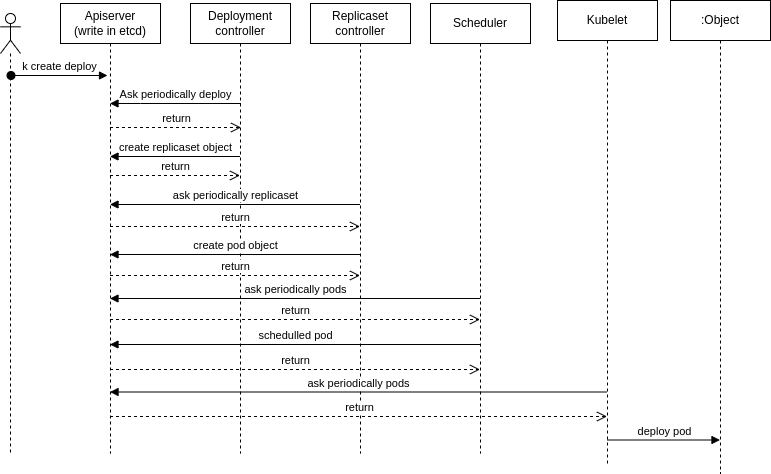
\includegraphics[width=1\linewidth]{assets/k8s-deploy-creation-drawio.png}
\end{frame}


\section{k8s, Pods and co}
\subsection{k8s, How to deploy}

\subsubsection{Pods command}
\begin{frame}[fragile]{\subsubsecname}
\begin{itemize}
  \item \textbf{(po) minimal}: \texttt{k run <pod\_name> --image=<image\_name>}
  \item \textbf{(po) example}: \texttt{k run toto-frontend --image=nginx -l "app=toto,tier=frontend" --dry-run=client -o yaml}
  \item \textbf{(po) connection}: \texttt{k exec -it <pod\_name> -- <command>}
  \item \textbf{(po) interaction}: \texttt{k [get|describe|edit|delete] [pods|po] <pods\_name>}
  \begin{itemize}
    \item in \texttt{get} command ready: container in pod ready/container total in pod
  \end{itemize}
  \item \textbf{(po) edition} can only edit 4 field (if edit anything else: delete/recreate)
  \begin{itemize}
    \item spec.containers[*].image
    \item spec.initContainers[*].image
    \item spec.activeDeadlineSeconds
    \item spec.tolerations
  \end{itemize}
  \item \textbf{(po) get yaml} \texttt{k get pods <pods\_name> -o yaml > <pods\_name>.po.yaml}
  \item \textbf{(po) create from yaml} \texttt{k apply -f <pods\_name>.po.yaml}
  \item \textbf{(po) delete from yaml} \texttt{k delete -f <pods\_name>.po.yaml}
\end{itemize}

\end{frame}

\subsubsection{Replicasets and Deployments}
\begin{frame}{Replicasets and Deployments}

  \begin{itemize}
    \item \textbf{(rs) interaction}: \texttt{k [get|describe|edit|delete] [replicasets|rs] <rs\_name>}
    \item \textbf{(ds) interaction}: \texttt{k [get|describe|edit|delete] [daemonsets|ds] <ds\_name>}
    \item \textbf{(deploy) minimal}: \texttt{k create deploy <deploy\_name> --image=<image\_name>}
    \item \textbf{(deploy) interaction}: \texttt{k [get|describe|edit|delete] [deployments|deploy] <deploy\_name>}
    \item \textbf{(rs|deploy) scaling}: \texttt{k scale [rs|deploy] <rs|deploy\_name> --replicas=<number>}
    \item free edition for rs and deploy
    \begin{itemize}
      \item after rs edition need to delete pod to create new version
      \item deploy have update policy
    \end{itemize}
    \item replicasets: be sure to have the good number of a pod
    \item daemonsets: be sure to have the pod on all node
    \item deployment: be sure to have the pod as defined
  \end{itemize}
  
\end{frame}

\subsubsection{Yaml comparaison}
\begin{frame}[fragile]{Yaml comparaison}

\begin{small}
\begin{columns}
  \begin{column}{0.20\linewidth}
    \textbf{toto.po.yaml}
    \begin{lstlisting}








apiVersion: v1
kind: Pod
metadata:
  labels:
    run: toto
  name: toto
spec:
  containers:
  - image: nginx
    name: toto
    \end{lstlisting}
  \end{column}
  \begin{column}{0.27\linewidth}
    \textbf{toto.rs.yaml}
    \begin{lstlisting}
apiVersion: apps/v1
kind: ReplicaSet
metadata:
  labels:
    app: toto
  name: toto
spec:
  selector:
    matchLabels:
      app: toto
  template:
    metadata:
      labels:
        app: toto
    spec:
      containers:
      - image: nginx
        name: nginx
  replicas: 1
  \end{lstlisting}
  \end{column}
  \begin{column}{0.26\linewidth}
    \textbf{toto.ds.yaml}
    \begin{lstlisting}
apiVersion: apps/v1
kind: DaemonSet
metadata:
  labels:
    k8s-app: ingress
  name: kube-proxy
spec:
  selector:
    matchLabels:
      k8s-app: ingress
  template:
    metadata:
      labels:
        k8s-app: ingress
    spec:
      containers:
      - image: nginx
        name: nginx
    \end{lstlisting}
  \end{column}
  \begin{column}{0.27\linewidth}
    \textbf{toto.deploy.yaml}
    \begin{lstlisting}
    apiVersion: apps/v1
    kind: Deployment
    metadata:
      labels:
        app: toto
      name: toto
    spec:
      selector:
        matchLabels:
          app: toto
      template:
        metadata:
          labels:
            app: toto
        spec:
          containers:
          - image: nginx
            name: nginx
      replicas: 1
    \end{lstlisting}
  \end{column}
\end{columns}
\end{small}
\end{frame}

\subsubsection{Multicontainer Pod}
\begin{frame}[fragile]{\subsubsecname}
  \begin{itemize}
  \item sidecar (log, metric scraper)
  \item adapter
  \item ambassador
  \end{itemize}
\end{frame}

\subsubsection{Kubectl proxy and port forward}
\begin{frame}[fragile]{Kubectl proxy and port forward}
  \begin{itemize}
  \item If you try to access apiserver, you need authent
  \item \texttt{kubectl proxy}: permit to acces apiserver and expose in on localhost:8001
  \item \texttt{curl http://localhost:8001/api/v1/namespaces/default/services/nginx/proxy/}
  \item unless exposition you cannot access pod from outside the cluster
  \item \texttt{kubectl port-forward service/nginx 28080:80}
  \item can be use pod, deploy, svc
  \end{itemize}
\end{frame}


\subsection{k8s, How to list}

\subsubsection{Kubectl version tricks}
\begin{frame}[fragile]{\subsubsecname}
  \begin{itemize}
    \item \texttt{k versions}: cluster version
    \item \texttt{k api-versions}: all version supported by the cluster
    \item \texttt{k api-resources}: list ressource, shortcut, apigroup
    \item \texttt{k explain <resource>}: describe a resource and give recommended version
    \item \texttt{k explain <resource> --recursive}: give all key off a resource
  \end{itemize}
\end{frame}

\subsubsection{Kubectl output format}
\begin{frame}[fragile]{\subsubsecname}
  \begin{itemize}
    \item \texttt{k get <resource>}: list the resource
    \item \texttt{k get <resource> <specific resource>}: retourn only the specific resource targeted
    \item \texttt{k get <resource> -o wide}: generally give more detail
    \item \texttt{k get <resource> -o json}: return data in json format
    \item \texttt{k get po nginx -o yaml}: return data in yaml format
    \item \texttt{k get <resource> --show-labels}: show labels in the list
  \end{itemize}
  Good but not detailed here
  \begin{itemize}
    \item \texttt{k get <resource> -o jsonpath='{.items[*].metadata.name}'}
    \item \texttt{k get no -o jsonpath='{.items[?(@.metadata.name == "node01")].status.nodeInfo.osImage}'}
    \item \texttt{k get no -o custom-columns='NAME:.metadata.name, OS:.status.nodeInfo.osImage'}: print column of your choice
    \item \texttt{k get po -l "tier=front,app=ldap"}: filter by label
  \end{itemize}
\end{frame}


\subsection{k8s, Command and args}

\subsubsection{Command and args}
\begin{frame}[fragile]{\subsubsecname}
  \begin{itemize}
    \item \texttt{command} in yaml file will surcharge \texttt{entrypoint} in dockerfile
    \item \texttt{args} in yaml file will surcharge \texttt{command} in dockerfile
  \end{itemize}
  \begin{lstlisting}
    ---
    apiVersion: v1
    kind: Pod
    metadata:
      labels:
        run: toto
      name: toto
    spec:
      containers:
      - image: ubuntu
        name: toto
        command:
        - sleep
        args:
        - "1200"
\end{lstlisting}
\end{frame}


\subsection{k8s, Storage}

\subsubsection{Storage architecture}
\begin{frame}[fragile]{\subsubsecname}
  \begin{itemize}
    \item \texttt{volumeMount} connect a pod to a \texttt{volume}
    \item \texttt{volume} is linked to a \texttt{Persistent Volume Claim} (not only)
    \item \texttt{PVC} claim the reservation of a \texttt{Persistent Volume}
    \item \texttt{PVC} constraint are
    \begin{itemize}
      \item sufficient Capacity
      \item Access Modes
      \item Volumes Modes
      \item (Storage Class)
      \item (Selector)
    \end{itemize}
    \item \texttt{PV} give a place to store
    \item \texttt{Storage Class} generate dynamically \texttt{Persistent Volume}
  \end{itemize}
\end{frame}

\subsubsection{Storage implementation}
\begin{frame}[fragile]{Storage implementation}
\begin{small}
\begin{columns}
  \begin{column}{0.33\linewidth}
    \begin{lstlisting}
---
apiVersion: v1
kind: Pod
metadata:
  labels:
    run: toto
  name: toto
spec:
  containers:
  - image: ubuntu
    name: toto
    volumeMounts: # <----
    - mountPath: /opt
      name: data-volume
  volumes: # <----
  - name: data-volume
    persistentVolumeClaim: # <----
      claimName: myclaim
    \end{lstlisting}
  \end{column}

  \begin{column}{0.33\linewidth}
    \begin{lstlisting}
---
apiVersion: v1
kind: PersistentVolumeClaim # <----
metadata:
  name: myclaim
spec:
  accessModes:
    - ReadWriteOnce
  resources:
    requests:
      storage: 500Mi
    \end{lstlisting}
  \end{column}

  \begin{column}{0.33\linewidth}
    \begin{lstlisting}
---
apiVersion: v1
kind: PersistentVolume # <----
metadata:
  name: pv-vol1
spec:
  # ReadOnlyMany, ReadWriteOnce, ReadWriteMany
  accessModes:
    - ReadWriteMany
  capacity:
    storage: 12Gi
  # or replace with storage provider
  hostPath:
    path: /tmp/data
  # Retain or Recycle or Delete
  persistentVolumeReclaimPolicy: Retain
      \end{lstlisting}
  \end{column}
\end{columns}
\end{small}
\end{frame}


\subsection{k8s, Envvars, config map and secret}


\subsubsection{Envvars and Configmap}
\begin{frame}[fragile]{\subsubsecname}
  \begin{itemize}
    \item \texttt{k create [configmap|cm] app-config --from-literal="APP\_CONFIG=blue" --from-literal="APP\_MODE=prod"}
    \item \texttt{kubectl create configmap app-config --from-file=app\_config.properties}
  \end{itemize}
  \begin{lstlisting}
    ---
    apiVersion: v1
    kind: ConfigMap
    metadata:
      name: app-config
    data:
      APP_COLOR: blue
      APP_MODE: prod
  \end{lstlisting}
\end{frame}

\begin{frame}[fragile]{Configmap in pod}
  \begin{lstlisting}
    [...]
    kind: Pod
    spec:
      containers:
      - image: ubuntu
        name: toto
        # envvars
        env:
        - name: my_super_var
          value: 42
        - name: POD_NAME
          valueFrom:
            fieldRef:
              fieldPath: metadata.name
        # V1
        - name: APP_COLOR
          valueFrom:
            configMapKeyRef:
              name: app-config
              key: APP_COLOR
        # V2
        envFrom:
        - configMapRef:
            name: app-config
        # V3
        volumeMounts:
        # ...
      volumes:
      - name: app-config-volume
        configMap:
          name: app-config
  \end{lstlisting}
\end{frame}


\subsubsection{Envvars and Configmap}
\begin{frame}[fragile]{Secret}
  \begin{itemize}
    \item \texttt{k create secret [generic|docker-registry|tls] app-secret --from-literal="APP\_CONFIG=blue" --from-literal="APP\_MODE=prod"}
    \item \texttt{kubectl create secret [generic|docker-registry|tls] app-secret --from-file=app\_config.properties}
  \end{itemize}
  \begin{lstlisting}
    [...]
    kind: Pod
    spec:
      containers:
      - image: ubuntu
        name: toto
        # envvars
        env:
        # V1
        - name: APP_COLOR
          valueFrom:
            secretKeyRef:
              name: app-config
              key: APP_COLOR
        # V2
        envFrom:
        - secretRef:
          name: app-secret
        # V3
        volumeMounts:
        # ...
      volumes:
      - name: secret-volume
        secret:
          secretName: dotfile-secret
  \end{lstlisting}
\end{frame}


\subsection{k8s, Pod accessibility}


\subsubsection{Service}
\begin{frame}[fragile]{\subsubsecname}
  \begin{itemize}
    \item
    \item \texttt{k expose [po|rs|sts|deploy] <resource\_name> --port=<pod\_number>}: minimal
    \item \texttt{k expose deploy poulet --port=80 --target-port=80 --type=ClusterIP --name=tchoutchou}
  \end{itemize}
  \begin{itemize}
    \item Service Type: ClusterIP (Default), NodePort, LoadBalancer (on cluster provider)
    \item Port's option: port (service's port), target-port (pod's port), nodeport (port on the node, on all node)
  \end{itemize}
  \begin{lstlisting}
  \end{lstlisting}
\end{frame}


\subsubsection{Ingress}
\begin{frame}[fragile]{\subsubsecname}
  \begin{itemize}
    \item need an ingress controller
    \item to interface a fqdn or a subdomain to a service
    \item \texttt{k create ingress <ingress-name> --rule="host/path=service:port"}
    \item \texttt{k create ingress ingress-test --rule="wear.my-online-store.com/wear*=wear-service:80"}
  \end{itemize}
  \begin{lstlisting}
    ---
    apiVersion: networking.k8s.io/v1
    kind: Ingress
    metadata:
      name: ingress-test
    spec:
      rules: # can be multiple in an only ingress
      - host: wear.my-online-store.com
        http:
          paths:
          - backend:
              service:
                name: wear-service
                port:
                  number: 80
            path: /wear
            pathType: Prefix
  \end{lstlisting}
\end{frame}


\section{k8s, Not Concerning Pod}
\subsection{k8s, Authorization}


\subsubsection{User and certificats}
\begin{frame}[fragile]{User}
  \begin{itemize}
    \item End User
    \item Developer
    \item Administrator
    \item Automatizator, Bot
  \end{itemize}
  \begin{itemize}
    \item https://github.com/mmumshad/kubernetes-the-hard-way/blob/master/tools/kubernetes-certs-checker.xlsx
    \item Client:
      \begin{itemize}
        \item api-server - etcd
        \item controller-manager - api-server
        \item scheduller - api-server
        \item api-server - kubelet (for each node)
        \item kube-proxy - api-server (for each pod)
        \item User
      \end{itemize}
    \item Server:
      \begin{itemize}
        \item etcd
        \item api-server
        \item kubelet
      \end{itemize}
    \item CA
      \begin{itemize}
        \item etcd
        \item kubernetes
      \end{itemize}
  \end{itemize}
  \begin{lstlisting}
  \end{lstlisting}
\end{frame}

\begin{frame}[fragile]{CSR}
  \begin{itemize}
    \item \texttt{openssl genrsa -out jane.key 2048}: generate user private key
    \item \texttt{openssl req -new -key -subj '/CN=jane' -out jane.csr}: Generate Certificate Signing Request
    \item \texttt{k apply -f jane.csr.yml}: after create kube csr
    \item \texttt{k get csr}
    \item \texttt{k certificate deny jane}
    \item \texttt{k certificate approve jane}
    \item then bind a role to the user
  \end{itemize}
  \begin{lstlisting}
  ---
  # jane.csr.yml
  apiVersion: certificates.k8s.io/v1
  kind: CertificateSigningRequest
  metadata:
    name: jane
  spec:
    groups:
    - system:authenticated
    # cat jane.csr | base64
    request: LS0tLS1CRUdJTiBDRVJUSUZJQ0FURSBSRVFVRVNULS0tLS0KTUlJQ1ZqQ0NBVDRDQVFBd0VURVBNQTBHQTFVRUF3d0dZV3R6YUdGNU1JSUJJakFOQmdrcWhraUc5dzBCQVFFRgpBQU9DQVE4QU1JSUJDZ0tDQVFFQXY4azZTTE9HVzcrV3JwUUhITnI2TGFROTJhVmQ1blNLajR6UEhsNUlJYVdlCmJ4RU9JYkNmRkhKKzlIOE1RaS9hbCswcEkwR2xpYnlmTXozL2lGSWF3eGVXNFA3bDJjK1g0L0lqOXZQVC9jU3UKMDAya2ZvV0xUUkpQbWtKaVVuQTRpSGxZNDdmYkpQZDhIRGFuWHM3bnFoenVvTnZLbWhwL2twZUVvaHd5MFRVMAo5bzdvcjJWb1hWZTVyUnNoMms4dzV2TlVPL3BBdEk4VkRydUhCYzRxaHM3MDI1ZTZTUXFDeHUyOHNhTDh1blJQCkR6V2ZsNVpLcTVpdlJNeFQrcUo0UGpBL2pHV2d6QVliL1hDQXRrRVJyNlMwak9XaEw1Q0ErVU1BQmd5a1c5emQKTmlXbnJZUEdqVWh1WjZBeWJ1VzMxMjRqdlFvbndRRUprNEdoayt2SU53SURBUUFCb0FBd0RRWUpLb1pJaHZjTgpBUUVMQlFBRGdnRUJBQi94dDZ2d2EweWZHZFpKZ1k2ZDRUZEFtN2ZiTHRqUE15OHByTi9WZEdxN25oVDNUUE5zCjEwRFFaVGN6T21hTjVTZmpTaVAvaDRZQzQ0QjhFMll5Szg4Z2lDaUVEWDNlaDFYZnB3bnlJMVBDVE1mYys3cWUKMkJZTGJWSitRY040MDU4YituK24wMy9oVkN4L1VRRFhvc2w4Z2hOaHhGck9zRUtuVExiWHRsK29jQ0RtN3I3UwpUYTFkbWtFWCtWUnFJYXFGSDd1dDJveHgxcHdCdnJEeGUvV2cybXNqdHJZUXJ3eDJmQnErQ2Z1dm1sVS9rME4rCml3MEFjbVJsMy9veTdqR3ptMXdqdTJvNG4zSDNKQ25SbE41SnIyQkZTcFVQU3dCL1lUZ1ZobHVMNmwwRERxS3MKNTdYcEYxcjZWdmJmbTRldkhDNnJCSnNiZmI2ZU1KejZPMUU9Ci0tLS0tRU5EIENFUlRJRklDQVRFIFJFUVVFU1QtLS0tLQo=
    signerName: kubernetes.io/kube-apiserver-client
    usages:
    - client auth
  \end{lstlisting}
\end{frame}


\subsubsection{User and certificats}
\begin{frame}[fragile]{User}
  \begin{itemize}
    \item \texttt{k create [serviceaccount|sa] <sa\_name>}: create service account
    \item \texttt{k create sa toto}: create service account
    \item \texttt{kubectl create role <role_name> --verb=<verb_list> --resource=<resources>}: create role
    \item \texttt{kubectl create role toto --verb=get,list,watch --resource=rs,deploy}: create role
    \item \texttt{k create rolebinding admin --clusterrole=admin --user=user1 --user=user2 --group=group1 --serviceaccount=toto}: create role
    \item \texttt{}
  \end{itemize}
  \begin{lstlisting}
  \end{lstlisting}
\end{frame}


% Todo
\subsection{k8s, Network Policies}

\begin{frame}[fragile]{Todo}
\begin{itemize}
\item[todo] Kubectl proxy and port forward (ckad)(cks)
\item[app access] service (Nodeport, clusterIp) (ckad)(cka)
* DNS (cka)
* Ingress (ckad)(cka)(cks)
\item[config] Config map (ckad)(cka)
* Env vars (ckad)(cka)
* Secrets (generic, docker-registry) (ckad)(cka)
\item[scheduling] namespace (ckad)(cka)
* Rolling update and rollback (ckad)(cka)
* Taint and toleration (ckad)(cka)
* Node affinity (ckad)(cka)
* Node selector (ckad)(cka)
\item[vrac] Logs (ckad)(cka)
* Blue Green deployment (ckad)
* Canary Deployment (ckad)
* Jobs (ckad)
* CronJob (ckad)
* initcontainer (cka)
* Security context (ckad)(cka)(cks)
* etcd (cka)
* Scheduling (cka)
* Metrics (ckad)
* Cluster port (cka)
* Request and limits (in pods and limitrange) (ckad)(cka)
* Cluster update (cka)(cks)
* Cluster install (cka)
* Cluster Backup and restore (cka)
* Security primitive (cka)(ckS)
* k8s certificate (cka)(cks)
* Certificate Signing Request CSR (cka)(cka)
* API Group (ckad)(cka)(cks)
* Authorization (ckad)(cka)(cks)
* Role Base RBAC (ckad)(cka)(cks)
* Cluster Role (ckad)(cka)(cks)
* Service Account (ckad)(cka)(cka)
* Default Admission Controller (ckad)(cks)
* Validating and Mutating Admission Controllers (ckad)(cks)
* Network Policy NetPol (ckad)(cka)(cks)
* Kubeconfig (ckad)(cka)(cks)
* API Version (ckad)
* CNI (cka)
* ReadinessProbe and LivenessProbe (ckad)
* Docker Image (ckad)
* Operator Framework (CRD + Custom Controller) (ckad)
* Helm (ckad)
* Authentication (cka)(cks)
\item[security] CIS Linux (cks)
* CIS k8s (cks)
* Kube bench (cks)
* TLS (cka)(cks)
* Kubelet security (cks)
* Dashboard (cks)
* Securing Dashboard (cks)
* Docker service conf and securing (cks)
* Limite node access (cks)
* SSH Hardening (cks)
* Kernel Module Restriction (cks)
* Disable Port (cks)
* Firewall Basics (cks)
* Syscalls and seccomp (cks)
* Syscalls - AquaSec Tracee (cks)
* AppArmor (cks)
* Pod Security Policy PSP (cks)
* Open Policy Agent (cks)
* Secret Management (cks)
* gVisor (cks)
* kataContainer (cks)
* Runtime class (cks)
* One way SSL, mutual SSL (cks)
* image policy webhook (cks)
* Kubesec (cks)
* Trivy (cks)
* Falco (cks)
* Immutability (cks)
* Audit log (cks)
\end{itemize}
\end{frame}


\section{Sonarcube}

\subsection{sonar, theorie}

\subsubsection{Quality}
\begin{frame}[fragile]{What's hiding behind quality}
  7 axes of quality (Technical Dept)
  \begin{itemize}
    \item Coding rules
    \item Complexity
    \item Duplications
    \item Potential Bugs/Security Problems
    \item Test Coverage
    \item Architecture Design
    \item Comment
  \end{itemize}
\end{frame}

\subsubsection{What s about sonar}
\begin{frame}[fragile]{\subsubsecname}
  \begin{tabular}{p{.1cm} p{8cm} p{.1cm}}
    & \begin{center} "Sonar is the central place to manage code quality, offering visual reporting on and accross projects and enabling to replay the past to follow metrics evolution" \end{center} & \\
    & \begin{center} source http://www.sonarsource.org/ \end{center} & \\
  \end{tabular}
\end{frame}


\subsection{sonar, usage}

\subsubsection{I need an instance}
\begin{frame}[fragile]{\subsubsecname}
  \begin{itemize}
    \item \texttt{docker run --rm --stop-timeout 3600 sonarqube}: just to launch
    \item \texttt{docker run --rm -p 9000:9000 --stop-timeout 3600 sonarqube}: to see something on \texttt{http://localhost:9000}
    \item \texttt{docker run --rm -p 9000:9000 --stop-timeout 3600 -v \$(pwd)/data:/opt/sonarqube/data sonarqube}: to save data
    \item \texttt{docker run --rm -p 80:9000 -v /opt/sonar/data:/opt/sonarqube/data -v /opt/sonar/logs:/opt/sonarqube/logs -v /opt/sonar/extensions:/opt/sonarqube/extensions sonarqube}: to save evrithing
    \item More info on \texttt{https://hub.docker.com/\_/sonarqube}
  \end{itemize}
\end{frame}

\subsubsection{How an dev use it}
\begin{frame}[fragile]{\subsubsecname}
  Sonar scanner management
  \begin{itemize}
    \item Developers commit and push on the repository
    \item CI server call sonar scanner (can be done in local too)
    \item Sonar scanner ask sonar server which rules to applies
    \item Sonar scanner scan and return result to sonar server
    \begin{itemize}
      \item Can add additional information as result of UT
      \item Can add annotation to disable rules on particular files
    \end{itemize}
  \end{itemize}
\end{frame}

\subsubsection{How an admin use it}
\begin{frame}[fragile]{\subsubsecname}
  Sonar server management
  \begin{itemize}
    \item Project: manual or from repository, a lot of config as:
    \begin{itemize}
      \item short term branch: only scan new modification
      \item long term branch: scan full repository
    \end{itemize}
    \item Issues: Detected Problem's Dashboard
    \item Rules: What will be check during scanner (organised by repository)
    \item Quality Profile: Group a list of rules and affect a severity (Info, Minor, Major, Critical, Blocker) on each
    \begin{itemize}
      \item \texttt{Bulk Change} button permit to activate all filtered rules in a profile
    \end{itemize}
    \item Quality Gates: Criteria which defined if the project is clean enougth or not, default
    \begin{itemize}
      \item Coverage is less than 80%
      \item Duplicated Lines is greater than 3%
      \item Maintainability Rating is worse than A
      \item Reliability Rating is worse than A
      \item Security Hotspots Reviewed is less than 100%
      \item Security Rating is worse than A
      \item Non comprehensive
    \end{itemize}
  \end{itemize}
\end{frame}


\section{Shell}

\subsection{Shell, Bash - Bourne Again Shell}

\subsubsection{Shell}
\begin{frame}[fragile]{\subsubsecname}
  \begin{itemize}
    \item \texttt{shell}: generally used to designate a command line interpreter that can access services and interact with the kernel of an operating system
    \item \texttt{role}: process a command line, understand its contents and perform the associated task
    \item \texttt{sh}: Bourne Shell
    \item \texttt{bash}: Bourne Again Shell
    \item \texttt{csh}: C-Shell (near to C synthax)
    \item \texttt{tcsh}: TENEX C-Shell
    \item \texttt{zsh}: Z-Shell
    \item ect.
  \end{itemize}
\end{frame}

\subsubsection{Bash - Files}
\begin{frame}[fragile]{\subsubsecname}
  \begin{itemize}
    \item \texttt{(file) \textasciitilde{}/.bashrc}: permit to customize your prompt
    \item \texttt{(file) \$HOME/.bash\_alias}: permit to load alias and variables on each terminal
    \item \texttt{(command) history}: bash keep your command history
    \item \texttt{(file) \$HOME/.bash\_history}: same as the command \item \texttt{history}
    \item \texttt{(file) \$HOME/.profile}: read if \item \texttt{\$HOME/.bash\_profile} or \texttt{\$HOME/.bash\_login} do not exist. Get new path for the PATH environment variable.
  \end{itemize}
\end{frame}

\subsubsection{Bash - Scripting}
\begin{frame}[fragile]{\subsubsecname}
  \begin{itemize}
    \item \texttt{Variable}: init, use print (do not forget double quote), arrays, dictionaries
    \item \texttt{Loop}: for, while, do, done
    \item \texttt{Condition}: if, then, elif, fi, conditional execution
    \item \texttt{Brace expansion}: \texttt{cp \{a,b\}.js}
    \item \texttt{Shell execution}: with backquote or \$()
    \item \texttt{Parameter}: substitution
    \item \texttt{Functions}
  \end{itemize}
\end{frame}

\subsubsection{Bash - Substitution}
\begin{frame}[fragile]{\subsubsecname}
  \begin{itemize}
    \item \texttt{Basics}
    \begin{itemize}
      \item name='John'
      \item echo \$\{name\}
      \item echo \$\{name/J/j\} $=>$ `john' (substitution)
      \item echo \$\{name:0:2\} $=>$ `Jo' (slicing)
      \item echo \$\{name:0:length\} $=>$ `Jo' (slicing with length=2)
      \item echo \$\{name::2\} $=>$ `Jo' (slicing)
      \item echo \$\{name::-1\} $=>$ `Joh' (slicing)
      \item echo \$\{name:(-1)\} $=>$ `n' (slicing from right)
      \item echo \$\{name:(-2):1\} $=>$ `h' (slicing from right)
      \item echo \$\{food:-Cake\} $=>$ \$food or `Cake'
    \end{itemize}
    \item \texttt{File path}
    \begin{itemize}
      \item STR=`/path/to/foo.cpp'
      \item echo \$\{STR\%.cpp\} $=>$ /path/to/foo
      \item echo \$\{STR\%.cpp\}.o $=>$ /path/to/foo.o
      \item echo \$\{STR\%/*\} $=>$ /path/to
      \item echo \$\{STR\#\#*.\} $=>$ cpp (extension)
      \item echo \$\{STR\#\#*/\} $=>$ foo.cpp (basepath)
      \item echo \$\{STR\#*/\} $=>$ path/to/foo.cpp
      \item echo \$\{STR/foo/bar\} $=>$ /path/to/bar.cpp
    \end{itemize}
  \end{itemize}
\end{frame}

\begin{frame}[fragile]{\subsubsecname}
  \begin{itemize}
    \item \texttt{Substitution}
    \begin{itemize}
      \item \$\{FOO\%suffix\} Remove suffix
      \item \$\{FOO\#prefix\} Remove prefix
      \item \$\{FOO\%\%suffix\} Remove long suffix
      \item \$\{FOO\#\#prefix\} Remove long prefix
      \item \$\{FOO/from/to\} Replace first match
      \item \$\{FOO//from/to\} Replace all
      \item \$\{FOO/\%from/to\} Replace suffix
      \item \$\{FOO/\#from/to\} Replace prefix
    \end{itemize}
    \item \texttt{Manipulation}
    \begin{itemize}
      \item echo \$\{STR,\} $=>$ lowercase 1st letter
      \item echo \$\{STR,,\} $=>$ all lowercase
      \item echo \$\{STR\textasciicircum{}\} $=>$ uppercase 1st letter
      \item echo \$\{STR\textasciicircum{}\textasciicircum{}\} $=>$ all uppercase
    \end{itemize}
  \end{itemize}
\end{frame}

\subsubsection{Bash - Functions}
\begin{frame}[fragile]{\subsubsecname}
  \begin{lstlisting}
# function is not mandatory
function myfunc() {
  echo "hello $1"
}
if myfunc; then
  echo "success"
else
  # to raise errors
  echo "failure"
fi
  \end{lstlisting}
  \begin{itemize}
    \item \$\# Number of arguments
    \item \$\* All positional arguments (as a single word)
    \item \$\@ All positional arguments (as separate strings)
    \item \$1 First argument
    \item \$\_ Last argument of the previous command
  \end{itemize}
\end{frame}

\subsubsection{Bash - Options}
\begin{frame}[fragile]{\subsubsecname}
  \begin{itemize}
    \item Options
    \begin{itemize}
      \item set -o noclobber \# Avoid overlay files ($echo 'hi' > foo$)
      \item set -o errexit \# Used to exit upon error, avoiding cascading errors
      \item set -o pipefail \# Unveils hidden failures
      \item set -o nounset \# Exposes unset variables
    \end{itemize}
    \item Glob options
    \begin{itemize}
      \item shopt
      \item shopt -s nullglob \# Non-matching globs are removed  ('*.foo' $=>$ '')
      \item shopt -s failglob \# Non-matching globs throw errors
      \item shopt -s nocaseglob \# Case insensitive globs
      \item shopt -s dotglob \# Wildcards match dotfiles ($'{}*.sh' => '.foo.sh'$)
      \item shopt -s globstar \# Allow ** for recursive matches ($'lib/**/*.rb' => 'lib/a/b/c.rb'$)
    \end{itemize}
  \end{itemize}
\end{frame}

\subsubsection{Bash - Miscelanous}
\begin{frame}[fragile]{\subsubsecname}
  \begin{itemize}
    \item Comment
    \begin{itemize}
      \item \texttt{\# Single line comment}
      \item \texttt{' You can make this comment on multiline '}
    \end{itemize}
    \item \$\{\#FOO\} $=>$ Length of FOO
    \item Default values
    \begin{itemize}
      \item \$\{FOO:-val\} \$FOO, or val if unset (or null)
      \item \$\{FOO:=val\} Set \$FOO to val if unset (or null)
      \item \$\{FOO:+val\} val if \$FOO is set (and not null)
      \item \$\{FOO:?message\} Show error message and exit if \$FOO is unset (or null)
      \item Omitting the \texttt{:} removes the (non)nullity checks
    \end{itemize}
    \item source: https://devhints.io/bash
  \end{itemize}
\end{frame}


\subsection{Shell, Zsh - Z-Shell}

\subsubsection{Zsh - Files}
\begin{frame}[fragile]{\subsubsecname}
  \begin{itemize}
    \item \texttt{shell}: generally used to designate a command line interpreter that can access services and interact with the kernel of an operating system
    \item \texttt{/etc/zshenv}: Always run for every zsh.
    \item \texttt{\textasciitilde{}/.zshenv}: Usually run for every zsh (see below).
    \item \texttt{/etc/zprofile}: Run for login shells.
    \item \texttt{\textasciitilde{}/.zprofile}: Run for login shells.
    \item \texttt{/etc/zshrc}: Run for interactive shells.
    \item \texttt{\textasciitilde{}/.zshrc}: Run for interactive shells.
    \item \texttt{/etc/zlogin}: Run for login shells.
    \item \texttt{\textasciitilde{}/.zlogin}: Run for login shells.
  \end{itemize}
\end{frame}

\subsubsection{Zsh - History - Pushd}
\begin{frame}[fragile]{\subsubsecname}
  \begin{itemize}
    %\item \texttt{shell}: generally used to designate a command line interpreter that can access services and interact with the kernel of an operating system
    \item Configurable history
    \begin{itemize}
      \item \texttt{HISTSIZE=1000}
      \item \texttt{SAVEHIST=1000}
      \item \texttt{HISTFILE=\textasciitilde{}/.history}
    \end{itemize}
    \item Pushd extension
    \begin{itemize}
      \item \texttt{pushd}: stock your dir
      \item bash stock 2 directory, zsh stock more (20+)
      \item \texttt{popd}
      \item \texttt{dirs}: list saved dirs
      \item \texttt{dirs -v}: like dirs but with number
      \item \texttt{cd -1}: go to dir number 1
      \item \texttt{1}: alias for \texttt{cd -1}
    \end{itemize}
  \end{itemize}
\end{frame}

\subsubsection{Zsh - Completion}
\begin{frame}[fragile]{\subsubsecname}
  \begin{itemize}
    \item \texttt{bash}
    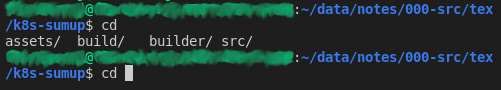
\includegraphics[width=1\linewidth]{assets/shell-bash-completion.png}
    \item \texttt{zsh}
    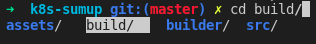
\includegraphics[width=1\linewidth]{assets/shell-zsh-completion.png}
  \end{itemize}
\end{frame}

\subsubsection{Zsh - Aliases}
\begin{frame}[fragile]{\subsubsecname}
  \begin{itemize}
    \item Alias suffixe
      \begin{itemize}
        \item \texttt{alias -s pdf=\"evince \"}: Permit to launch \texttt{./fichier.pdf} instead of \texttt{evince ./fichier.pdf}
      \end{itemize}
    \item Alias globaux
      \begin{itemize}
        \item \texttt{alias -g G=$'$ $|$ grep $'$}: Permit to launch \texttt{ls /bin G zsh} instead of \texttt{ls /bin $|$ grep zsh}
      \end{itemize}
  \end{itemize}
\end{frame}

\subsubsection{Zsh - Options}
\begin{frame}[fragile]{\subsubsecname}
  \begin{itemize}
    \item $setops/nosetops$ active or unactive an option
    \item $NO\_BEEP$: set, that annoying beep goes away,
    \item $NO\_LIST\_BEEP$:, beeping is only turned off for ambiguous completions,
    \item $AUTO\_CD$: You can change directory without $cd$
    \item $CD\_ABLE\_VARS$: If you $cd foo$ and there is no directory $foo$, zsh will try to $cd  \$foo$
    \item $CORRECT, CORRECT\_ALL$: zsh will check if you miss spells your command
    \item Examples:
    \begin{itemize}
    \item setopt glob bareglobqual nullglob rcexpandparam extendedglob unset
    \item unsetopt markdirs globsubst shwordsplit shglob ksharrays cshnullglob
    \item unsetopt allexport aliases errexit octalzeroes
    \end{itemize}
  \end{itemize}
\end{frame}


\subsection{Shell, Oh my Zsh}

\subsubsection{Zsh - Oh-my-zsh}
\begin{frame}[fragile]{\subsubsecname}
  \begin{itemize}
    \item Multiple theme/prompt customisazion
    \item Oh-my-zsh \#1 (https://github.com/ohmyzsh/ohmyzsh)
    \item Cheatsheet: https://github.com/ohmyzsh/ohmyzsh/wiki/Cheatsheet
    \item Alias
    \begin{itemize}
      \item \texttt{alias}:	List all aliases
      \item \texttt{take / mkcd}:	Create a new directory and change to it, will create intermediate directories as required.
      \item \texttt{zsh\_stats}:	Get a list of the top 20 commands and how many times they have been run.
      \item \texttt{md}: mkdir -p
      \item \texttt{rd}: rmdir
      \item \texttt{..}: cd ..
      \item \texttt{...}: cd ../..
      \item \texttt{....}: cd ../../..
      \item \texttt{.....}: cd ../../../..
      \item \texttt{/}: cd /
      \item \texttt{d}: dirs -v (lists last visited directories)
      \item \texttt{cd +n}: Switch to directory number n
      \item \texttt{-}: cd to last visited directory
      \item \texttt{1}: cd -1
      \item \texttt{2}: cd -2
      \item \texttt{3}: cd -3
      \item \texttt{4}: cd -4
      \item \texttt{5}: cd -5
      \item \texttt{6}: cd -6
      \item \texttt{7}: cd -7
      \item \texttt{8}: cd -8
      \item \texttt{9}: cd -9
    \end{itemize}
  \end{itemize}
\end{frame}

\subsubsection{Zsh - Plugins}
\begin{frame}[fragile]{\subsubsecname}
  \begin{itemize}
    \item https://github.com/ohmyzsh/ohmyzsh/tree/master/plugins
    \item https://github.com/ohmyzsh/ohmyzsh/wiki/Plugins-Overview
    \item Plugins (313 the 2022.04.29)
      \begin{itemize}
        \item 1password
        \item ansible
        \item bazel
        \item branch
        \item cp: cp with progress bar (rsync)
        \item docker, docker-compose
        \item git, git-auto-fetch, git-flow
        \item golang
        \item helm
        \item history, history-substring-search
        \item kubectl, kubectx, kube-ps1
        \item npm, npx
        \item pip, pip-env, pyenv, pylint
        \item poetry
        \item redis-cli
        \item screen, tmux
        \item vault
        \item wakeonlan
        \item z
      \end{itemize}
    \item Add
      \begin{itemize}
        \item Conf ()
        \item Alias
        \item Autocompletion
      \end{itemize}
  \end{itemize}
\end{frame}

\subsubsection{Zsh - Plugins - Z bash}
\begin{frame}[fragile]{\subsubsecname}
  \begin{itemize}
    \item https://github.com/rupa/z
    \item For bash or zsh
    \item Stat on browse directory (rank/date)
    \item cd to most pertinent
    \item Command
    \begin{itemize}
      \item z part\_of\_the\_name
      \item z -e part\_of\_the\_name: echo the best match
      \item z -l part\_of\_the\_name: list all match by frequency
      \item z foo bar: cd to most frecent dir matching foo, then bar
    \end{itemize}
    \item Options
    \begin{itemize}
      \item Set \$\_Z\_CMD to change the command name (default z).
      \item Set \$\_Z\_DATA to change the datafile (default \$HOME/.z).
      \item Set \$\_Z\_MAX\_SCORE  lower  to  age  entries  out faster (default 9000).
      \item Set \$\_Z\_NO\_RESOLVE\_SYMLINKS to prevent symlink resolution.
      \item Set \$\_Z\_NO\_PROMPT\_COMMAND to handle PROMPT\_COMMAND/precmd yourself.
      \item Set \$\_Z\_EXCLUDE\_DIRS to an array of directory trees to exclude.
    \end{itemize}
  \end{itemize}
\end{frame}


\subsection{Shell, p10k}

\subsubsection{Zsh - Plugins - p10k}
\begin{frame}[fragile]{\subsubsecname}
  \begin{itemize}
    \item https://github.com/romkatv/powerlevel10k
    \item For zsh
    \item (Git) Add indicator for edited file
    \item Same theme as zsh
    \item Permit to customize left and right prompt
    \item Existing segments
    \begin{itemize}
      \item command\_execution\_time: duration (wall time) of the last command
      \item disk\_usage: disk usage
      \item goenv: go environment from goenv
      \item go\_version: go version
      \item ip: IP address and bandwidth usage for a specified network interface
      \item java\_version: java version
      \item kubecontext: current kubernetes context
      \item load: CPU load
      \item nordvpn: nordvpn connection status
      \item os\_icon: your OS logo (apple for macOS, swirl for debian, etc.)
      \item package: name@version from package.json
      \item ram: free RAM
      \item status: exit code of the last command
      \item swap: used swap
      \item time: current time
      \item vcs: Git repository status
      \item vim\_shell: vim shell (:sh)
      \item virtualenv: python environment from venv
      \item wifi: WiFi speed
    \end{itemize}
  \end{itemize}
\end{frame}

\subsubsection{Zsh - Completion}
\begin{frame}[fragile]{\subsubsecname}
  \begin{itemize}
    \item \texttt{bash}
    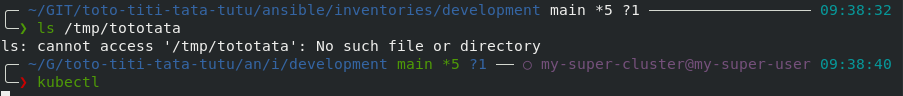
\includegraphics[width=1\linewidth]{assets/shell-p10k-auto_segment.png}
    \item Auto show context
    \item Auto hide useless path
  \end{itemize}
\end{frame}

\subsubsection{Zsh - Plugins - p10k}
\begin{frame}[fragile]{\subsubsecname}
  \begin{itemize}
  \item to make your custom segment you need to begin your function by $prompt$
  \item it is recommend to begin by $my\_$ to avoid future conflict
  \begin{lstlisting}
function prompt_my_cpu_temp() {
  integer cpu_temp="$(</sys/class/thermal/thermal_zone0/temp) / 1000"
  if (( cpu_temp >= 80 )); then
    p10k segment -s HOT -f red -t "${cpu_temp}"
  elif (( cpu_temp >= 60 )); then
    p10k segment -s WARN -f yellow -t "${cpu_temp}"
  fi
}
  \end{lstlisting}
  \item then add $my\_cpu\_temp$ to
  \begin{itemize}
    \item $POWERLEVEL9K\_RIGHT\_PROMPT\_ELEMENTS$
    \item or $POWERLEVEL9K\_LEFT\_PROMPT\_ELEMENTS$
  \end{itemize}
\end{itemize}
\end{frame}


\subsection{Tilt}

\subsubsection{Tilt - Intro}
\begin{frame}[fragile]{\subsubsecname}
  \begin{itemize}
    \item https://tilt.dev/
    \item Smart rebuilds and live reloads
    \item docker, docker-compose, k8s oriented
    \item Tilt devoloped in Go, Tiltfile are writen in Starlack (dialect of Python)
    \item https://docs.tilt.dev/cli/tilt\_completion\_bash.html: autocompletion
    \item https://docs.tilt.dev/api.html: All functions, cli, types, data, etc
    \item Examples
    \begin{itemize}
      \item https://github.com/tilt-dev/tilt-avatars/blob/main/Tiltfile: full app
      \item https://docs.tilt.dev/snippets.html
      \begin{itemize}
        \item docker build
        \item deploy k8s, with yaml, with kustomize, with helm
        \item run local command to use result
        \item make port-forward
        \item configure k8s resources
        \item create k8s resource from existing objects
        \item deploy docker-compose
        \item run go/node server
        \item show k8s logs
        \item build image and use it to deploy in k8s
        \item manage per-developer customizations
      \end{itemize}
      \item https://docs.tilt.dev/
      \begin{itemize}
        \item Exemples for Statix HTML, Go, Node, Python, Java, C\#, Bazel
      \end{itemize}
    \end{itemize}
\end{itemize}
\end{frame}

\subsubsection{Tilt - Docker\_build}
\begin{frame}[fragile]{\subsubsecname}
  \begin{itemize}
    \item  docker\_build
  \end{itemize}
  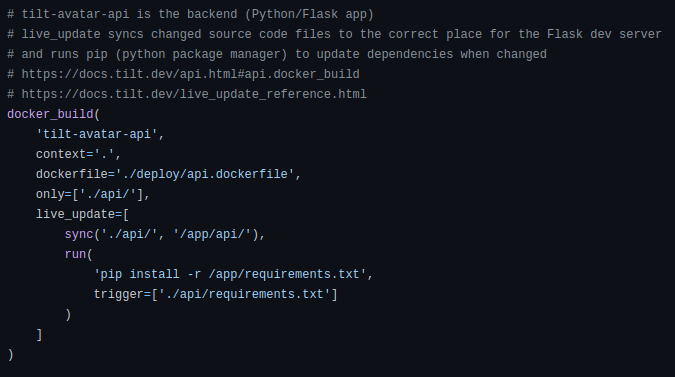
\includegraphics[width=1\linewidth]{assets/tilt-func-build-docker.png}
\end{frame}

\subsubsection{Tilt - K8s deployment}
\begin{frame}[fragile]{\subsubsecname}
  \begin{itemize}
    \item  k8s\_yaml and k8s\_resource
  \end{itemize}
  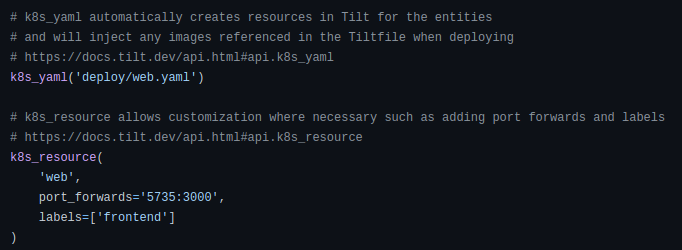
\includegraphics[width=1\linewidth]{assets/tilt-func-k8s_deploy}
\end{frame}

\subsubsection{Tilt - K8s deployment}
\begin{frame}[fragile]{\subsubsecname}
  \begin{itemize}
    \item local: launch script in local
    \item local\_resource: launch script in local
    \begin{itemize}
      \item cmd: install dependencies
      \item debs: files to watch
      \item serve\_cmd: launch service
    \end{itemize}
    \item os.getenv: read env variable
  \end{itemize}
\end{frame}


\end{document}
